%	This subsection provides some info on the controllers that run on AtlantikSolar

\begin{figure}[tb]
    \centering
     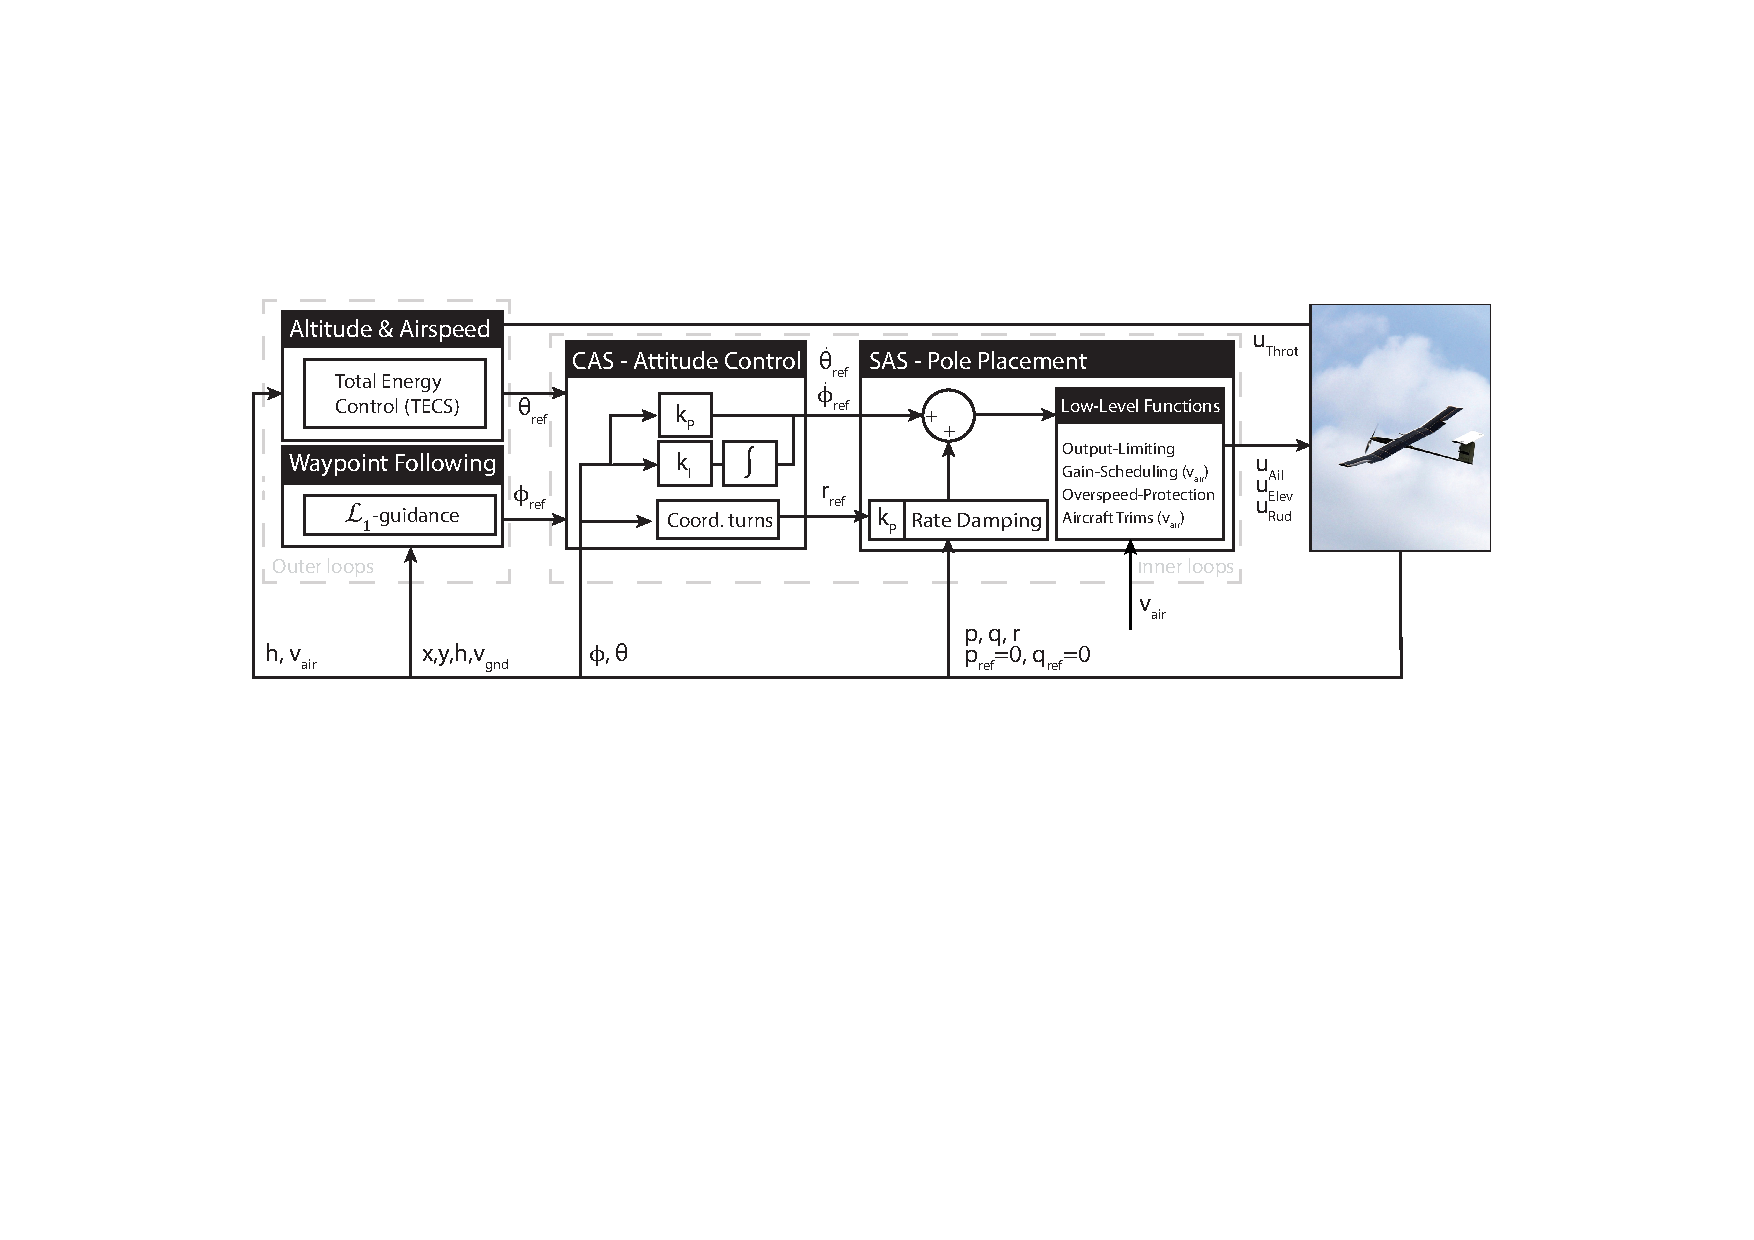
\includegraphics[width=\linewidth]{images/11_ControlScheme/ControlScheme.pdf}
    \caption{Control Scheme implemented for AtlantikSolar.}
    \label{fig:ControlScheme}
\end{figure}

AtlantikSolar features autonomous navigation up to the level of loithering through user--defined waypoints. The complete control structure (Fig.~\ref{fig:ControlScheme}) is offline tuned based on the identified system model (Sec.~\ref{sec:SystemID}), functionality is tested in an X--Plane 10 Hardware--In--the--Loop (HIL) simulation and finally refined in extensive flight tests. For inner--loop control, our baseline--solution corresponds to a set of cascaded saturated PID controllers: the Stability Augmentation System (SAS) applies rate--damping to shape the airplane's frequency respons, while the Control Augmentation System (CAS) applies proportional--integral feedback to achieve roll ($\phi$) and pitch ($\theta$) reference tracking. As a cascaded approach, proper tuning requires iteration of the gains to achieve maximum performance and robustness against model uncertainties and external disturbances. Flight tests showed that due to AtlantikSolar's high wingspan and thus high inertial ($I_z$ and $I_x$ especially), coordinated turn control s essential to smoothen the adverse yaw behaviour and achieve the no--sidelslip yaw rate $r=\frac{g\cdot \sin(\phi)}{v_{air}}$. To avoid overload of the highly optimized structure, output limiters and an over--speed protection are applied. Furthermore, the control actions are in a final stage adapted with respect to the dynamic pressure $q=\frac{1}{2}\rho v^{2}_{air}$ and essentially accounting for the change of the effective moments created by the control surfaces. 

Once the inner--loops are well tuned, waypoint navigation control synthesis is enabled. AtlantikSolar employs a $\mathcal{L}_1$ nonlinear guidance law which commands the lateral acceleration of the vehicle based on a look--ahead distance $\mathcal{L}_1$ as noted in the equation below:

\begin{eqnarray}
 a_{s_{ref}} &=& 2\frac{V_T^2}{L_1}\sin \eta
\end{eqnarray}
which is subsequently translated to roll references while consistent dynamic behaviour is achieved via adaptation of the look--ahead distance as in~\cite{L1stabAnalysis}. This guidance law is integrated into our control structure as described in~\cite{OMLAS_MED_14} and combined with an extended version of the Pixhawk Open--Source Total Enery Control System (TECS)~\cite{PixhawkWebsite} to achieve altitude reference tracking: First, a slew rate constraint on the reference altitude $h_{ref}$ has been integrated to reach smoother altitude control at pre-definable climb and sink rates, which is especially important for low propulsion-power to weight-ratio UAVs such as AtlantikSolar. Second, we've implemented ``thermal compliance'': In an updraft, the standard TECS implementation will decrease $\theta_{ref}$ to decrease the altitude if $h>h_{ref}$. To allow gaining potential energy from a thermal, we perform gain-scheduling on $k_{SW}$ (the TECS pitch loop ``speed-weight'' parameter), to make TECS use $\theta_{ref}$ fully and only for airspeed control and $u_{Throt}$ only for altitude control. When at $h>h_{ref}$, the plane will thus keep $\theta_{ref}=\theta_{ref}(t)$  such that $v(t)=v_{ref}(t)$ and will gradually disable the motor, potentially gaining altitude for strong thermals. Furthermore, altitude protection measures has been implemented, i.e. full throttle is forced for $h<h_{min}$, at $h>h_{max}$ we re-schedule $k_{SW}$ to gradually allow a pitch-down and thus altitude decrease again, and at $h>h_{max}+50m$ the controller automatically engages the spoilers for maximum descend rate. The inner PID-based pitch- and roll control loops are executed at a sampling period of $T_{SAS,CAS}=0.01s$, while the high-level $\mathcal{L}_1$\&TECS controllers run with $T_{\mathcal{L}_1,TECS}=0.05s$. Given these settings, the full controller requires less than 4\% CPU load, 5KB of RAM and 47KB Flash memory and is thus computationally lightweight when compared to other Pixhawk applications (see~\cite{OMLAS_MED_14}) such as the state estimation. The whole control application is designed to be modular, and noteworthy more sophisticated approaches like model-predictive control~\cite{OMLAS_MED_14} and robust $H_\infty$--based controllers~\cite{Mosimann_FT} for inner loop control have been implemented and flown on test planes in addition to the aforementioned PID--baseline inner--loop control solution. 